\chapter{FaPS Networking}
\label{ch:faps-networking}

\author{Nico Kratky}
%
FaPS Networking is a custom UDP-based library that is mainly used for communication between FaPS (see \ref{ch:faps}) and different kinds of client, eg. FaPS-save (see \ref{ch:faps-save}) and the NodeJS server (see
\ref{sec:webserver}).

\section{TCP vs UDP in real time environments}

Both TCP and UDP are members of the transport layer of the internet protocol suite, commonly known as the TCP/IP stack \cite{rfc1122}.

\subsection{Connection-Oriented and Connectionless Protocols}

There are two groups of protocols. The ones that require setting up a logical connection before data can be exchanged and the ones that don't require a link between the two communication partners. They are also called
\textit{connection-oriented transport services} (COTS) and \textit{connectionless transport services} (CLTS) \cite{connectionbased-vs-connectionless}. The advantages and disadvantes of both are important to know when choosing one of these types of protocols.
The main feature of COTS is that it is reliable, meaning that the protocol will ensure that sent messages are received reliably and in order. As discussed in \ref{ch:realtimesystems} it is not that big of a deal for
real-time applications if packets are dropped, therefor a CLTS was chosen.

\subsection{Perfomance}

As perfomance is a critical component of real-time applications, some research had to be conducted to get the best possible result.

This research included the comparison of the packet headers. As seen in figures \ref{fig:tcp-header} and \ref{fig:udp-header} it is clearly visible that the TCP header is much larger the the UDP header. In fact, TCP requires 20 bytes and UDP requires only 8 bytes for the header information.

\begin{figure}[H]
    \centering
    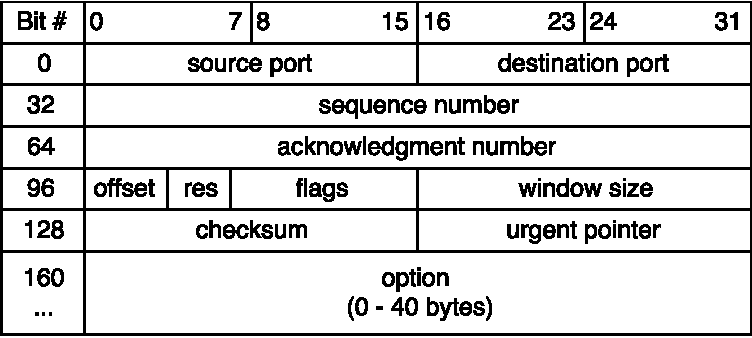
\includegraphics[width=8cm,keepaspectratio]{tcp-header}
    \caption{Header found in a TCP packet}
    \label{fig:tcp-header}
\end{figure}

\begin{figure}[H]
    \centering
    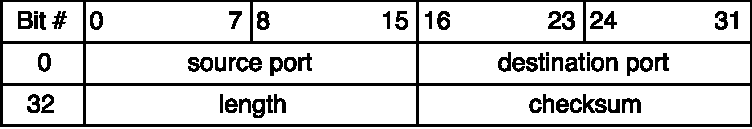
\includegraphics[width=8cm,keepaspectratio]{udp-header}
    \caption{Header found in a UDP datagram}
    \label{fig:udp-header}
\end{figure}

TCP also has a built-in feedback mechanism which checks if all packets are received by the communication partner and if they are received in order. This mechanisms not only produces a lot of overhead, but also is the data
most likely outdated when it is resent. Therefor it is not a problem if such packets are dropped.

Considering all these factors the decision to use UDP over TCP was made. TCP is a great protocol for example for sending large files where it is necessary that all bytes come in order and reliably. If one byte is missing
then the whole file would be corrupt. UDP however is a lot better for transferring time critical information as it produces less overhead \cite{TCPUDPRTlifesize}.

\section {Handling Connections}

As UDP is a connectionless protocols, neither does it know if the other end of the communacation is ready to receive data nor if it is even existing. Therefor a way of handling connections using UDP had to implemented.

The core of this implementation is a map. A map is a associative container that is available through C++'s STL (Standard Template Library). This maps contains all clients as keys, and the associated timestamps of the last
received keepalive message as values.

After starting the server, two threads are started. The first one handles all incoming messages. If a received message is a keepalive message the timestamp of the client that sent this message is update
to the current time. The second thread monitors these timestamps. If the difference between the current timestamp and the stored timestamp of a client exceeds 1.5 seconds, the client is declared disconnected and removed
from the list.

Also when a client is instantiaed a thread is started to handle the keepalive messages. The only task of this thread is to send a keepalive message to the server and then wait one second. All of this is done in a loop that
only finishes when the clients deconstructor is called, thus disconnects.

\section {Handshake}

The handshake procedure is a very important part of connecting. This makes sure that the server is notified whenever a client is waiting to connect.

When the server receives a connection request (see \ref{tab:faps-networking-control-messages}), it has to check if it can accept further clients. This limit is set as a static constant in the \textit{Server} class. The
default value is \textbf{8}. If this check is successful the server sends an acknowledgement message to the client. If the check fails, the client will receive a connection refused message. In this implementation the
clients connect call will block until it is connected. This is done by a loop that will be exited once the server sends an acknowledgement. In between the connection attempts one second is waited.

These two procedures can be both seen in the code listings (\ref{lst:faps-networking-handshake-server} and \ref{lst:faps-networking-handshake-client}) and the sequence diagram (\ref{fig:faps-networking-handshake}) below.

\begin{minipage}{\linewidth}
\begin{lstlisting}[caption={Server handshake method}, label=lst:faps-networking-handshake-server, captionpos=b, language=C++]
void Server::shake_hands(boost::asio::ip::udp::endpoint& remote) {
    if (endpoints_.size() < MAX_CLIENTS_) {
        send(control_messages["ACKNOWLEDGE"], remote);
        endpoints_[remote] = std::chrono::system_clock::now();
    }
    else {
        send(control_messages["CONNECTION_REFUSED"], remote);
    }
}
\end{lstlisting}
\end{minipage}

\begin{minipage}{\linewidth}
\begin{lstlisting}[caption={Client handshake method}, label=lst:faps-networking-handshake-client, captionpos=b, language=C++]
void Client::connect() {
    while (!connected) {
        send(control_messages["CONNECTION_REQUEST"]);

        std::string reply;
        receive(reply);

        if (reply.compare(control_messages["ACKNOWLEDGE"]) == 0) {
            connected = true;

            std::thread t_keepalive{&Client::keepalive, this};
            t_keepalive.detach();
        }
        else {
            std::this_thread::sleep_for(TIMEOUT_);
        }
    }
}
\end{lstlisting}
\end{minipage}

\begin{figure}[H]
    \centering
    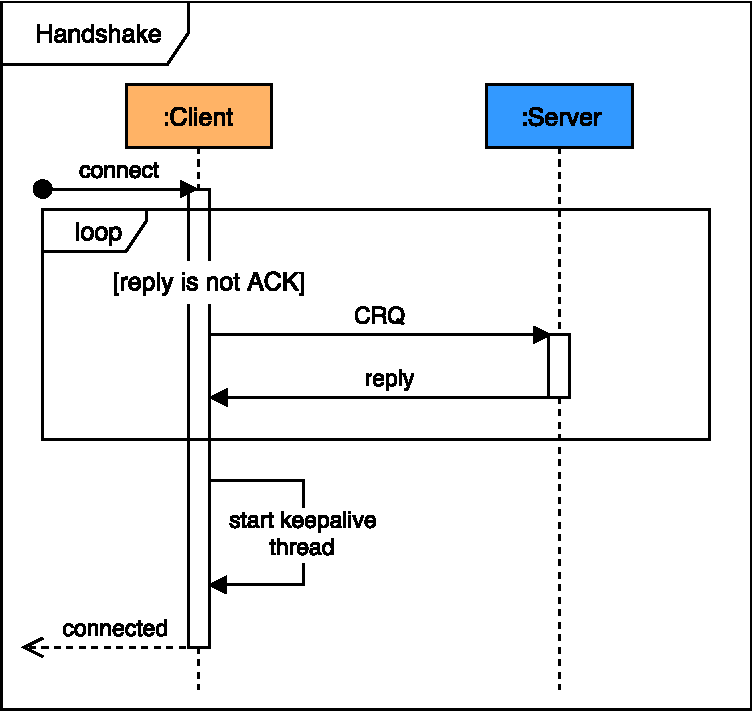
\includegraphics[width=8cm,keepaspectratio]{faps-networking-handshake}
    \caption{Handshake performed when a client tries to connect to server}
    \label{fig:faps-networking-handshake}
\end{figure}

\section{Control Message}

This table explains all control messages that can be exchanged.

\begin{table}[H]
    \centering
    \begin{tabular}{| l | l | p{5cm} |}
    \hline
    \textbf{Message} & \textbf{Sent to} & \textbf{Meaning} \\ \hline
    CRQ & server & Tells the server that a new client is waiting for the connection procedure \\ \hline
    ACK & client & Tells the client that the connection is acknowledged \\ \hline
    CRF & client & Tells the client that the server can not accept the connection \\ \hline
    KAV & server & Tells the server that the client is still alive and wants to stay connected \\
    \hline
    \end{tabular}
    \caption{Commands sent by one of the connection partners and what they do}
    \label{tab:faps-networking-control-messages}
\end{table}

